\documentclass{article}

\usepackage[margin=1in]{geometry}
\usepackage[center]{caption}
\usepackage{subfigure}
\usepackage{appendix}
\usepackage{amsmath}
\usepackage{graphicx}
\usepackage{todonotes}
\usepackage{tikz}

\usetikzlibrary{fit,positioning}

\newcommand{\HRule}{\rule{\linewidth}{0.1mm}}

\begin{document}

\title{ \HRule \\[0.2cm]
		Autonomous Agents\\ 
		Report Assignment 2: Single Agent Learning\\
		\HRule \\[0.1cm]
		}
		
\author{
		\emph{Authors:}\\[0.2cm]
		Agnes \textsc{van Belle} \small{ \emph{(10363130)}},\\ 
		Maaike \textsc{Fleuren} \small{ \emph{(10350470)}}, \\
		Norbert \textsc{Heijne} \small{ \emph{(10357769)}}, \\
		Lydia \textsc{Mennes} \small{ \emph{(10333843)}}
		}
		
\maketitle

\section{Introduction}
This report has been written for the Master Artificial Intelligence course Autonomous Agents. This report will contain the answers, motivation and explanation for our implementations of the tasks we had to accomplish in our second assignment for this course. These tasks were centered around the topic of `Single Agent Learning'.

\subsection{The environment} \label{sec:environment}
In all tasks there is assumed to be a grid world (of $11 \times 11$) with a predator and a prey in it. The agents can both move one tile forward each iteration. The direction they take (or if they move at all) is affected by probabilities (their policies). If they move over the edge of the grid they end up at the opposing side of the grid. The prey will never step onto the predator. We are focused on improving the decisions of one agent, the predator. 

\subsection{The state space representation} \label{sec:stateSpace}
In the experiments described the first report, we initially used a state space that was an intuitive, yet cumbersome representation. We referred to that state space representation as the `default' state space. The amount of states that was used in the default state space was $(11 \times 11) \times (11 \times 11) = 121 \times 121 = 14641$. We then changed the state space representation to a more efficient one, referred to as the `efficient' state space, which led to a reduction of 697 times less states, resulting in just 21 different states.

In this assignment, we used this efficient state space representation for the learning algorithms. To give a good understanding of our learning algorithms, which were built on the efficient state space representation, we will once again explain how this representation works.

Figure \ref{fig:statespaceSymm} illustrates that there is a symmetry in the default state space, and thus that there were relatively much values redundantly computed.
By using this symmetry in the default state space a much smaller state space was achieved. 

Each state represents a distance between the prey and predator. These are represented in the lower left diagonal of a matrix, in which the $x$-axis is the relative horizontal distance in the MDP and the $y$-axis the relative vertical distance in the MDP. This matrix is shown in Figure \ref{fig:NewStateRep}. Combinations of positions of prey and predator for which the horizontal and vertical distances are equal are now treated equivalent. 
Also two combinations for which the horizontal distance in one equals the vertical distance in the other and vice versa are considered equal. In order to navigate through this state space different actions are required. These are: \textit{horizontal retreat, horizontal approach, vertical retreat, vertical approach}, as illustrated in Figure \ref{fig:statespaceSymm}, and of course the action \textit{wait}. When interacting with the environment these actions are converted into corresponding actions in the real world. This only requires the relative direction of the prey (which is always located at the centre, regardless of its coordinates) with respect to the predator. This is computed by using the difference in location of the prey and predator on the $x$- and $y$-axis.

\begin{figure}[ht]
\centering
\subfigure[The $11 \times 11$ grid divided into eight symmetric pieces, with the corresponding possible moves which are also symmetric.]{
    \includegraphics[width=0.5\textwidth]{statespaceSymm.png}
    \label{fig:statespaceSymm}
}
\subfigure[Colormap of $V$-values, the brighter the color the higher the corresponding $V$-value. The prey is always located on the (1, 1) coordinate in this state representation.]{
    \includegraphics[width=0.4\textwidth]{VMatrixNewStateRep.png}
    \label{fig:NewStateRep}
}
\caption{Illustration of the symmetry and corresponding values of the new state space representation}
\label{fig:statespaceIll}
\end{figure}


\subsection{Implementation details}
This report will not be about our exact code and implementation details. However, a class diagram of our code is provided in Appendix \ref{app:classDiagram}.

\section{Learning algorithms}
As mentioned before, we will use the same environment as in the previous assignment. But in this assignment, we will assume the learning scenerio: the agent does not know the transition probabilities, nor the reward structure. On a very high level there are two ways to come to a good solution in this setting: learning the model, and do planning again (model based learning), or not learn the model, and directly try to learn a high-reward policy (model-free learning). In this assignment we will focus on the latter.\footnote{Roijers (2012) \textit{Assignments Autonomous Agents} p. 6}

\subsection{(M) Q-Learning}\label{sec:exercise1}
Q-Learning is an off-policy temporal-difference control algorithm. Temporal-difference methods can learn directly from raw experience without a model of the environment's dynamics. Furthermore, it updates estimates based in part on other learned estimates, without waiting for a final outcome.\footnote{Sutton, Barto (1998) \textit{Reinforcement Learning: An Introduction} Cambridge, Massachusetts: The MIT press. p. 133}

While the distinguishing feature of on-policy methods is that they estimate the value of a policy while using it for control, these two functions are separated in off-policy methods. The behavior policy, used to generate behavior, and the estimation policy, that is evaluated and improved, may in fact be unrelated. This separation is an advantage because the estimation policy may be deterministic (e.g., greedy), while the behavior policy can continue to sample all possible actions.\footnote{Sutton, Barto (1998) \textit{Reinforcement Learning: An Introduction} Cambridge, Massachusetts: The MIT press. p. 126} Its simplest form, \textit{one-step Q-learning}, is defined by\footnote{Sutton, Barto (1998) \textit{Reinforcement Learning: An Introduction} Cambridge, Massachusetts: The MIT press. p. 148}:
\begin{align*}
Q(s_t,a_t) & \leftarrow Q(s_t,a_t) + \alpha \left[ r_{t+1} + \gamma \displaystyle\max_a Q(s_{t+1},a) - Q(s_t,a_t) \right]
\end{align*}

For this assignment, we implemented Q-learning and used it for our predator agent. We used $\epsilon$-greedy action selection, which behaves greedily most of the time, but with probability $\epsilon$, instead select an action at random, uniformly, independently of the action-value estimates.\footnote{Sutton, Barto (1998) \textit{Reinforcement Learning: An Introduction} Cambridge, Massachusetts: The MIT press. p. 28} In this case, we used $\epsilon = 0.1$. We initiated the values of our Q-learning table optimistically with a value of 15 for all cells in the table.

Figure \ref{plot:QEalphagamma} shows plots on the performance of the agent over time for different $\alpha$ and for different $\gamma$ (discount factor) using $\epsilon$-greedy action selection.

%\begin{figure}
\missingfigure{Plots on the performance of the agent over time for different $\alpha$ and for different $\gamma$ (discount factor) using $\epsilon$-greedy action selection.} \label{plot:QEalphagamma}
%\end{figure}

\subsection{(M) Experiment with $\epsilon$ and optimistic initialization}\label{sec:exercise2}
\todo[inline, color=yellow]{Experiment with different values of $\epsilon$ and the optimistic initialization of the Q-table. Make up good values to test, and explain why you chose these values.}

\subsection{(SC) Softmax action selection instead of $\epsilon$-greedy}\label{sec:exercise3}
For this exercise, we did the same as we did in section \ref{sec:exercise1}, but instead of using $\epsilon$-greedy action selection we used softmax action selection. This means that the greedy action is still given the highest selection probability, but all the others are ranked and weighted according to their value estimates.\footnote{Sutton, Barto (1998) \textit{Reinforcement Learning: An Introduction} Cambridge, Massachusetts: The MIT press. p. 30}

Figure \ref{plot:QSalphagamma} shows plots on the performance of the agent over time for different $\alpha$ and for different $\gamma$ (discount factor), this time using softmax action selection.

%\begin{figure}
\missingfigure{Plots on the performance of the agent over time for different $\alpha$ and for different $\gamma$ (discount factor) using softmax action selection.} \label{plot:QSalphagamma}
%\end{figure}

\todo[inline, color=yellow]{Illustrate the difference between $\epsilon$-greedy and softmax, using graphs from your empirical results.}

\subsection{Other ways to do learning}

\subsubsection{(SC) On-policy Monte Carlo Control}\label{sec:exercise4.1}
As mentioned in section \ref{sec:exercise1}, on-policy methods try to evaluate or improve the policy that is used to make decisions.\footnote{Sutton, Barto (1998) \textit{Reinforcement Learning: An Introduction} Cambridge, Massachusetts: The MIT press. p. 122} Monte Carlo estimation can be used to approximate optimal policies, which results in Monte Carlo control. It proceeds according to the idea of generalized policy iteration, where one maintains both an approximate policy and an approximate value function. The value function is repeatedly altered to more closely approximate the value function for the current policy, and the policy is repeatedly improved with respect to the current value function.\footnote{Sutton, Barto (1998) \textit{Reinforcement Learning: An Introduction} Cambridge, Massachusetts: The MIT press. p. 118} In this case, our policy moves towards a softmax policy, which was previously explained in section \ref{sec:exercise3}. Furthermore, it is necessary to use exploring starts because making the policy greedy prevents further exploration of nongreedy actions.\\ 

\todo[inline, color=yellow]{Explain the difference with other learning methods theoretically, and compare them using informative graphs.}

\subsubsection{(SC) Off-Policy Monte Carlo Control}\label{sec:exercise4.2}
\textit{For an explanation off-policy methods, Monte Carlo control and softmax action selection, please take a look at section \ref{sec:exercise1}, \ref{sec:exercise4.1} and \ref{sec:exercise3} respectively.}
\\ \\ 
Off-policy Monte Carlo control follows the behavior policy while learning about and improving the estimation policy.\footnote{Sutton, Barto (1998) \textit{Reinforcement Learning: An Introduction} Cambridge, Massachusetts: The MIT press. p. 126}\\

\todo[inline, color=yellow]{Explain the difference with other learning methods theoretically, and compare them using informative graphs.}

\subsubsection{(SC) Sarsa}\label{sec:exercise4.3}
\textit{For an explanation of on-policy methods and temporal difference learning, please take a look at section \ref{sec:exercise1} or \ref{sec:exercise4.1}, and section \ref{sec:exercise1} respectively.}
\\ \\
In contrast to the Q-learning method, Sarsa is an on-policy temporal-difference control algorithm. Just like Q-learning it learns an action-value function rather than a state-value function, but for an on-policy method like Sarsa we must estimate $Q^\pi (s,a)$ for the current behavior policy $\pi$ and for all states $s$ and actions $a$.\footnote{Sutton, Barto (1998) \textit{Reinforcement Learning: An Introduction} Cambridge, Massachusetts: The MIT press. p. 145}

In Sarsa we consider transitions from state-action pair to state-action pair, and learn the value of state-action pairs. An alternating sequence of of states and state-action pairs forms an episode:

\begin{center}
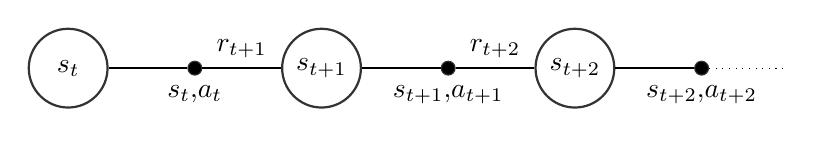
\begin{tikzpicture}
\tikzstyle{main}=[circle, minimum size = 10mm, thick, draw =black!80, node distance = 10mm]
\tikzstyle{connect}=[-, thick]
\tikzstyle{dot}=[circle, inner sep=0pt,minimum size=5pt, draw =black!80, fill=black, node distance = 10mm]
\tikzstyle{empty}=[rectangle, fill=white, node distance=10mm]
  \node[main, fill = white!100] (st) [] {$s_t$};
\node[dot] (stat) [right=of st, label=below:$s_t \text{,} a_t$] {};
  \node[main] (st1) [right=of stat] {$s_{t+1}$};
\node[dot] (st1at1) [right=of st1, label=below:$s_{t+1}\text{,} a_{t+1}$] {};
\node[main] (st2) [right=of st1at1] {$s_{t+2}$};
\node[dot] (st2at2) [right=of st2, label=below:$s_{t+2}\text{,} a_{t+2}$] {}; 
\node[empty] (empty) [right=of st2at2] {};

  \path (st) edge [connect] (stat)
        (stat) edge [connect] node[auto] {$r_{t+1}$} (st1)
	(st1) edge [connect] (st1at1)
	(st1at1) edge [connect] node[auto] {$r_{t+2}$} (st2)
	(st2) edge [connect] (st2at2);
\draw [dotted] (st2at2) -- (empty);
  \end{tikzpicture}
\end{center}

After every transition from a nonterminal state $s_t$ an update is done:

\begin{align*}
Q(s_t,a_t) & \leftarrow Q(s_t,a_t) + \alpha \left[ r_{t+1} + \gamma \, Q(s_{t+1},a_{t+1}) - Q(s_t,a_t) \right]
\end{align*}
If $s_{t+1}$ is terminal, then $Q(s_{t+1},a_{t+1})$ is defined as zero. As you can see, this update uses every element that makes up a transition from one state-action pair to the next ($s_t,a_t,r_{t+1},s_{t+1},a_{t+1}$), from which the name Sarsa originates.

\todo[inline, color=yellow]{Explain the difference with other learning methods theoretically, and compare them using informative graphs.}

\section{Conclusion}

\newpage
\nocite{*}
\bibliographystyle{plainnat}
\bibliography{references}

\newpage
\appendix
\appendixpage
\section{Class Diagram} \label{app:classDiagram}


\end{document}